\documentclass[pre,preprint]{revtex4-1}

% preamble:
\usepackage{appendix}
\usepackage{outline}
\usepackage{amsmath}    % need for subequations
\usepackage{graphicx}   % need for figures
\usepackage{verbatim}   % useful for program listings
\usepackage{color}      % use if color is used in text
\usepackage{subfigure}  % use for side-by-side figures
\usepackage{hyperref}   % use for hypertext links, including those to external documents and URLs
\raggedbottom           % don't add extra vertical space
\begin{comment}
\pagestyle{empty}       % use if page numbers not wanted
\end{comment}




\begin{document}

\title{The emergence of filament alignment and contraction in active filament networks}
\author{William McFadden, Edwin Munro}
\affiliation{University of Chicago, Institute for Biophysical Dynamics, Chicago, IL 60615}

\date{this day}


\begin{abstract}
We introduce a novel mechanisms of sorting and contraction in 2D networks of active bipolar filaments in the presence of activity gradients.  Our modeling framework is motivated by the gradients of myosin activity found in motile cells and cells undergoing cytokinesis.  We show that are sufficient to engrain engrain contractions even in the absence of asymmetric filament stiffness.  
\end{abstract}



\maketitle


\tableofcontents


















\section{Introduction}

































\section{Explanation of Model}

\subsection{Composite Cross-link \& Filament Representation}
We consider individual filaments as chains of springs with relaxed length $l_s$.  The orientations of neighboring springs are linearly coupled. Filaments can therefore be represented as a sequence of nodes with positions $\mathbf{x_i}$ and nearest neighbor interactions of the form

\begin{equation}
|F_{i,i+1}|_{\parallel} = -\mu\cdot\frac{|\mathbf{x_{i+1}}-\mathbf{x_i}|-l_s}{l_s} 
\end{equation}

\begin{equation}
|F_{i,i+2}|_{\perp} = -\frac{\kappa}{l_s^2}\cdot acos\left (\frac{\mathbf{x_{i+2}}-\mathbf{x_{i+1}}}{|\mathbf{x_{i+2}}-\mathbf{x_{i+1}}|} \cdot\frac{\mathbf{x_{i+1}}-\mathbf{x_i}}{|\mathbf{x_{i+1}}-\mathbf{x_i}|} \right ) 
\end{equation}


where, $\mu$ represents an extensional modulus of a filament, and $\kappa$ represents a bending modulus.   This is essentially a discretized equivalent to a model of filaments with separable extensional and bending moduli as in \cite{theo_hlm}.  We define the totally elastic force on a node as

\begin{equation}
\nabla{\cal H}_i =|F_{i,i+1}|_{\parallel} + |F_{i,i+2}|_{\perp}
\end{equation}

Here, we take the extensional modulus as a composite quantities related to both filament and cross-linker compliance in a manner similar to a recently proposed effective medium theory\cite{theo_crosslinknonlinear}.  In the limit of highly rigid cross-links and flexible filaments, our model reduces to the pure semi-flexible filament models of \cite{theo_hlm,theo_hlm2}.  In the opposite regime of nearly rigid filaments and highly flexible cross links, our method is still largely similar to the model of \cite{theo_crosslinknonlinear} in small strain regimes before any nonlinear cross link stiffening.  However, in departure from those models, the magnitude of the force on interior cross-links in our model is still the same as those on the exterior.  This is a simplification of the varying levels of strain that would actually be present in these cross-linkers as addressed in \cite{theo_crosslinknonlinear}, but we choose to ignore the slight variation in favor of an approximated, global mean approach.  

\begin{comment}Finally, in the event that the induced strain of the filament and the cross-linker are of comparable scales, our composite stiffness can be expressed by the approximation $huh$ as we shown in Appendix \ref{app:compos}.  In our simulations we explore the role that nonlinear stiffening of filaments or cross linkers would play, and what complications arise.\end{comment}



\subsection{2D Network Formation}

We choose to focus our attention on 2D networks both for their tractability as well as their relevance in the quasi-2D cytoskeletal cortex of many eukaryotic cells\cite{cellmech_flows}.  In addition, recent developments in 2D {\em in vitro} systems\cite{rheo_2D1,rheo_2D2}, make 2D models all the more interesting as a renewed focus of study.

We follow a mikado model approach by initializing a minimal network of connected unstressed linear filaments in a rectangular 2D domain.  We generate 2D networks of these semi-flexible filaments by laying down straight lines of length, $L$, with random position and orientation. We then assume that some fixed fraction of overlapping filaments become cross-linked (defined in \ref{exp_drag}) at their point of overlap.

Although real cytoskeletal networks may form with non-negligible anisotropy,  we  focus on isotropically initialized networks for simplicity.  We define the density using the average distance between cross-links along a filament, $l_c$. A simple geometrical argument can then be used to derive the number of filaments filling a domain as a function of $L$ and $l_c$\cite{theo_hlm}.  Here, we use the approximation that the number of filaments needed to tile a rectangular domain of size $W \times H$  is $2WH/Ll_c$, and that the length density is therefore $1/l_c$. 

In the absence of cross-link slip, we expect the network to form a connected solid with a well defined elastic modulus\cite{theo_hlm,theo_hlm2}.  These networks are only well-connected when the ratio of filament length to intercross-link spacing, $L/l_c$, is greater than $\sim 6$.  Near this percolation threshold, there are only locally connected domains, and discussions of global network properties becomes less reasonable.  Additionally, as the filament density is increased beyond this point, there is another transition between non-affine bending and affine stretching of filaments, which changes the dominating term of the network's elastic modulus.



\subsection{Drag-like Coupling Between Overlapping Filaments}
\label{exp_drag}
In contrast to previous models, we allow relaxation of the network's stored stress by letting the attachment points slip.  We do this by replacing an elastic interaction between pairs of points along filaments with a drag-like coupling between filaments.
\begin{equation}
\mathbf{F_{drag}} = \xi \cdot \int ds \: (\mathbf{v_i(s)}-\mathbf{v_j(s)}) \: p_{ij}(s)
\end{equation}

Where $p_{ij}(s)$ represents the locational distribution of cross-link points (equal to 1 at locations of cross-links and 0 elsewhere) and $\mathbf{v_i(s)}$ and $\mathbf{v_j(s)}$ represent the the velocities of the $i$th and $j$th filaments.  This model assumes a linear relation between applied force and the velocity difference between attached filaments.  Obviously, non-linearities can arise in the presence of force dependent detachment kinetics as well as non-linear force extension of cross-links. We address non-linear effects of stress induced unbinding in Appendix \ref{app:drag}.  Assuming inhomogeneities from non-linear effects are of second order, the motion for the entire network is governed by a dynamical equation of the form

\begin{equation}
\label{eqn:syst}
\int ds \: (\mathbf{\zeta v_i(s)} + \xi \sum _j(\mathbf{v_i(s)}-\mathbf{v_j(s)}) \: p_{ij}(s))= \nabla {\cal H}_i
\end{equation}

Here, the first term in the integral is the filament's intrinsic drag through its embedding fluid, $\zeta$, while the second comes from the drag-like coupling between filaments, $\xi$.  


\subsection{System of Equations for Applied Stress}
We model our full network as a coupled system of differential equations satisfying \ref{eqn:syst}.  Although the general mechanical response of this system may be very complex, we focus our attention on low frequency deformations and the steady-state creep response of the system to an applied stress.  To do this we introduce a fixed stress, $\sigma$ along the midline of our domain.  This stress points in the direction, $\mathbf{\hat{u}}$, producing either shear ($\mathbf{\hat{u}}=\mathbf{\hat{x}}$) or extensional ($\mathbf{\hat{u}}=\mathbf{\hat{y}}$) stress.

Finally, we add a 0 velocity constraint at the far edges of our domain of interest.  We assume that our network is in the "dry," low Reynold's number limit, where inertial effects are so small that we can equate our total force to 0.  Therefore, we have a dynamical system of wormlike chain filaments satisfying 

\begin{equation}
\int ds \: (\zeta\mathbf{v_i(s)} + \xi \sum _j(\mathbf{v_i(s)}-\mathbf{v_j(s)}) \: p_{ij}(s)) = \nabla {\cal H}_i + \sigma\mathbf{\hat{u(x)}}
\end{equation}

subject to constraints such that $\mathbf{v_i(x)}$ is 0 with $x=0$.  This results in an implicit differential equation for filament segments which can be discretized and integrated in time to produce a solution for the motion of the system.




\subsection{Incorporating Activity at Cross-link Points}

Discuss the modifications to the equations to add a motile force at points of overlap.




\subsection{Generating Activity Gradients}



































\section{Results}

\subsection{Steady-state Approximation of Effective Viscosity}
\label{sec:eff_vic}
We begin with a calculation of a strain rate estimate of the effective viscosity for a network described by our model in the limit of highly rigid filaments.  We carry this out by assuming we have applied a constant stress along a transect of the network.  With moderate stresses, we assume the network reaches a steady state affine creep. In this situation, we would find that the stress in the network exactly balances the sum of the drag-like forces from cross-link slip.  So for any transect of length D, we have a force balance equation.

\begin{equation}
\mathbf{\sigma} = \frac{1}{D}\sum_{filaments}\: \sum_{crosslinks}\xi \cdot (\mathbf{v_i(x)}-\mathbf{v_j(x)})
\end{equation}

where $\mathbf{v_i(x)}-\mathbf{v_j(x)}$ is the difference between the velocity of a filament, $i$, and the velocity of the filament, $j$, to which it is attached at the cross-link location, $\mathbf{x}$. We can convert the sum over cross-links to an integral over the length using the average density of cross-links, $1/l_c$ and invoking the assumption of (linear order) affine strain rate, $\mathbf{v_i(x)}-\mathbf{v_j(x)}=\dot \gamma x$. This results in

\begin{multline}
\mathbf{\sigma} =  \frac{1}{D}\sum_{filaments}\:  \int_0^L \xi \cdot  \: (\mathbf{v_i(s)}-\mathbf{v_j(s)}) \:\frac{ds \cos \theta }{l_c} \\
 = \sum_{filaments}\:  \frac{\xi \dot \gamma L}{l_c} \cos \theta \cdot (x_l + \frac{L}{2} \cos \theta)
\end{multline}

Here we have introduced the variables $x_l$, and $\theta$ to describe the leftmost endpoint and the angular orientation of a given filament respectively.  Next, to perform the sum over all filaments we convert this to an integral over all orientations and endpoints that intersect our line of stress. We assume for simplicity that filament stretch and filament alignment are negligible in this low strain approximation.  Therefore, the max distance for the leftmost endpoint is the length of a filament, L, and the maximum angle as a function of endpoint is $\arccos(x_l/L)$.  The linear density of endpoints is the constant $D/l_cL$ so our integrals can be rewritten as this density over $x_l$ and $\theta$ between our maximum and minimum allowed bounds.

\begin{equation}
\mathbf{\sigma} =  \frac{1}{D} \int_0^L dx_l \int_{-\arccos (\frac{x_l}{L})}^{\arccos (\frac{x_l}{L})}\frac{d\theta}{\pi} \frac{\xi \dot \gamma L}{l_c} \cdot \frac{D}{Ll_c}\cdot (x_l \cos \theta + \frac{L}{2} cos^2\theta)
\end{equation}

Carrying out the integrals and correcting for dangling filament ends leaves us with a relation between stress and strain rate.

\begin{equation}
\mathbf{\sigma} = \frac{(L-2l_c)^2 \xi}{4\pi l_c^2} \dot \gamma 
\end{equation}

We recognize the constant of proportionality between stress and strain rate as a viscosity.  Therefore, our approximation for the effective viscosity, $\eta_{eff}$, at steady state creep in this low strain limit is

\begin{equation}
\label{lin_eqn}
\eta_{eff} = \frac{(L-2l_c)^2 \xi}{4\pi l_c^2} .
\end{equation}

As illustrated in Figure \ref{fig:effvic}, under moderate strains ($\gamma<0.2$), our  simulations show that in the high density limit, our theoretical approximation from Eqn \ref{lin_eqn} is highly accurate at explaining the network behavior.  Aside from a geometrical factor, our approximation is valid for both shear and extensional stresses applied to the network.

As the density of the network approaches the breakdown limit, the effective viscosity diverges from our expected value.  At the low connectivities, our expected viscosity goes to 0, but the medium viscosity begins to take over as we cross the percolation threshold at $L/l_c \sim 6$.  
\begin{figure}[h!]
\centering
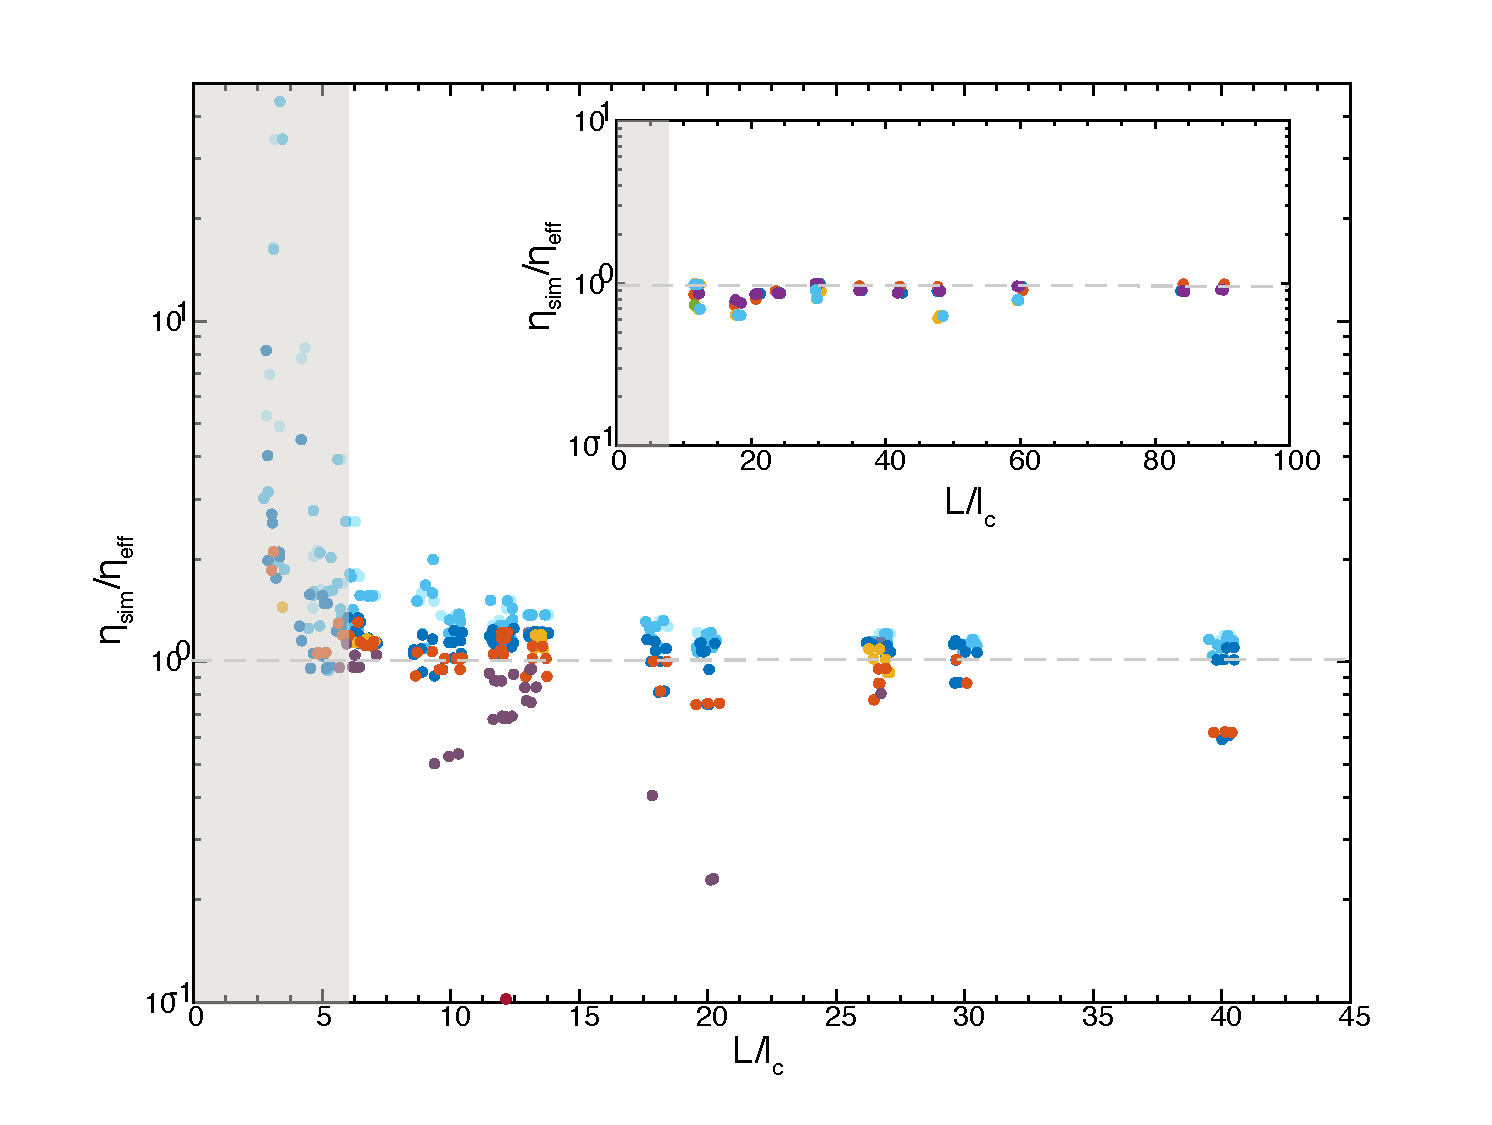
\includegraphics[width=\hsize]{eff_vic_master}
\caption{\label{fig:effvic}Ratio of effective viscosity measured by shear simulation to predicted effective viscosity as a function of connectivity, $L/l_c$. Inset: Same measurement for extensional simulations }
\end{figure}

In addition to changing the architecture and effective drag coefficient, we also validated the generality of our approximation by varying simulation size, medium viscosity, filament stiffness, and applied stress.  We were able to find a slight trend that depended on filament stiffness as indicated in the difference between blue and red data points in Figure \ref{fig:effvic}.  The deviation from our approximation and variability in results manifested itself more strongly when filaments were highly compliant.  To investigate this effect further, we next performed a more detailed analysis of the creep response while varying filament compliances.















\section{Summary and Conclusions}
We have proposed a simplified effective friction model for understanding 2D cross-linked networks. Our model extends previous Mikado and lattice models to include effects of cross-link relaxation. We expect that our model can confer insights into mechanisms of network stress relaxation in quasi-2D networks such as those found in \textit{in vitro} actin monolayer experiments\cite{rheo_2D1} as well as in eukaryotic actomyosin cortices\cite{cellmech_flows}.   

Our model is the first to address the plausible dependence of network effective viscosity on network structural properties.  This led to a derivation of an estimate for the long timescale creep rate of networks under constant stress.  Although this derivation neglects possible frequency dependence at short timescales, this finding offers a potential framework for addressing the dependence of network deformation rate on filament concentration and length.

Additionally, our simulations suggest that, in the presence of constant shear stress, cross-link friction will also produce a long-lived phase of sublinear creep as filaments relax from their affine stretched position. While this phase may transiently resemble more explicit 3D models such as \cite{theo_crosslinkslip1}, it is clear that our model differs by predicting that network will achieve a constant effective viscosity more rapidly.  In particular, we predict that this relaxation will occur at a rate similar to that of rate of cross-link slip derived strain and will therefore be negligible after the network has slipped by roughly ten times the magnitude of the purely affine mechanical deformation.  

In building our model we have neglected any other sources of potential mechanical relaxation in order to simplify out analysis. In the future, we hope to extend our model to include biochemically driven forms of relaxation such as filament turnover or regulated cross-link unbinding.

This model forms a basis for addressing 2D filament network deformation, and it proposes a simplified formulation of important qualitative properties. In this way we are able to address potentially general phases of network deformation and delineate what network properties may give rise to them.  This may provide an important starting point for addressing the general importance of network structure in more complex networks containing active elements. 



















\section{Acknowledgements}


















\appendix
\addappheadtotoc


\begin{comment}

\section{Network Tearing under Extensional Stress}


\subsection{Extensional Thinning and Network Tearing}

For moderate extensional stresses, the rigid filament approximation of the effective viscosity simply picks up a different geometrical factor out front.  

However, at higher stress and in the presence of different things happen.

\begin{equation}
\frac{\partial l_c}{dt}=l_c\dot \gamma =\frac{l_c \sigma}{\eta}\sim l_c^3\frac{ \sigma}{L^2 \xi}
\end{equation}

We can see that the rate of network thinning accelerates as we would expect.  When the network reaches some minimum connectivity we assume that it stops behaving as a continuum material and the network tears irreversibly.  

\begin{equation}
\tau_{break} = \frac{\eta_{eff}}{2\sigma}\cdot\left ( 1 -\frac{l_c^2}{l_{break}^2} \right )
\end{equation}

This provides us with an estimate of the timescale of catastrophic breakdown for a network with a given initial architecture and molecular drag.


\subsection{Tearing Events During Extensional Strain}

This behavior is caused primarily by the low density network undergoing tearing events that interrupt global connectedness.  

\end{comment}



\section{Deriving Molecular Drag Coefficients}
\label{app:drag}
Thus far, the idea of a molecular drag coefficient was taken as a phenomenological, measured parameter for a given experimental setup.  While this is a sufficient pragmatic justification, it's useful to try to motivate the quantitative value of this drag coefficient by connecting it to the underlying cross-link properties of binding affinity, concentration, and extensibility.

To do this we'll imagine the simplified case of two cross linkers sliding past each other in one dimension.  In this case, assume that we have an equilibrium number of bound cross-linkers, $n_B$, each of which is displaced from its equilibrium length by some distance $x$.  Each cross linker unbinds with rate $k_{off}$ and rebinds at it's relaxed position ($x=0$) with rate $k_{on}$.  At the same time, all the cross linkers are being pulled from their relaxed position at a rate, $v$, which is simply the rate at which the filaments are sliding past each other.  

We can write the differential equation for the change in the density of cross-links, $\rho$, at displacement $x$ as they are pulled upon, bind, and unbind.

\begin{equation}
\frac{\partial \rho}{\partial t} = -k_{off}\rho(x) - v\frac{\partial \rho}{\partial x} + k_{on}\delta(x)
\end{equation}

Recognizing that $\int \rho(x)=n_B$ implies $k_{on}=k_{off}n_B$, we can find the steady state solution

\begin{equation}
\rho(x) = \frac{n_b k_{off}}{v}\cdot exp\left ( -\frac{k_{off}}{v}x \right )
\end{equation}

If each cross-link has a spring constant $\mu_c$, then we can equate the force on all cross-links to the applied force that is sliding the filaments past each other.  Realistically, the spring constant and binding affinity would be functions of the cross-link stretch, but here we are taking them as approximately constant.  

\begin{equation}
\int_{0}^{\infty}\rho(x)\mu_cx dx = v \frac{\mu_c n_B}{k_{off}}= F_{app}
\end{equation}a

Therefore, the term next to v, (i.e. $\tfrac{\mu_c n_B}{k_{off}}$) would be equal to our molecular drag coefficient, $\xi$.  Assuming approximately 1 cross link per filament overlap, and using parameter estimates culled from Ferrer et al., we build the following table of estimates for $\xi$.

\begin{table}[h]
\begin{tabular}{| l | c | c |}
\hline
\textbf{cross-linker type} & $\alpha$-actinin & filamin-A  \\ \cline{1-1}
\textbf{dissociation constant ($s^{-1}$)} & 0.4 & 0.6 \\ \cline{1-1}
\textbf{spring constant ($nN / \mu m$)} & 455 & 820 \\ \cline{1-1}
\textbf{drag coefficient, $\xi$ ($\tfrac{nN \cdot s}{\mu m}$)} & 182 & 492 \\ 
\hline
\end{tabular}
\end{table}



This molecular description assumed both a constant off-rate and linear force extension of cross-links.  In the event that binding kinetics are regulated by the state of extension, we would expect (based on Rf) to find a region that exhibits a stick-slip behavior instead of the smooth.  Depending on the nature of any coupling between cross-links local stick-slip could either give rise to a global stick-slip behavior or a heterogenous mixture of stuck and sliding cross-links.  It would be interesting to explore this topic further in the future, but in the present analysis, we choose to ignore complications from these nonlinear effects.







\section{Computational Simulation Method}

We tested our analytical conclusions on a computational model.  More technical details of the model can be found in the Appendix, but we summarize the main modeling points here.

We discretize the filaments such that the equations of motion becomes a coupled system of equations for the velocities of filament endpoints, $\mathbf{x}$.  The drag-like force between overlapping filaments results in a coupling of the velocities of endpoints.  

\begin{equation}
\mathbf{A \cdot \dot x} = \mathbf{f(x)}
\end{equation}

where $\mathbf{A }$ represents a coupling matrix between endpoints of filaments that overlap, and $\mathbf{f(x)}$ is the spring force between pairs of filament segment endpoints.  We can then numerically integrate this system of equations to find the time evolution of the positions of all filament endpoints.

We generate a network by laying down filaments with random position and orientation within a domain of size $2D$ by $D$ with periodic boundaries in the y-dimension.  The external stress (shear or extensional/compressional) is applied to all filament endpoints falling within a fixed x-distance from the center of the domain.  Finally, filament endpoints falling within a fixed x-distance from the edges of the domain are constrained to be nonmoving.

\begin{figure}[h!]
\centering
\includegraphics[width=\hsize]{network_def}
\caption{\label{fig:sim}Two Simulation setups with $L=9 \mu m, D = 54 \mu m$ before (top) and after  (bottom) 1000 seconds of applied stress. a) low density $l_c=2 \mu m$, b) moderate density $l_c=1 \mu m.  $ Scale bar $ 20 \mu m$}
\end{figure}

The nominal units for length, force, and time are $\mu m$, nN, and s, respectively.  We explored parameter space around an estimate of biologically relevant parameter values, given in Table \ref{table:para}. 

\begin{table}[h]
\centering
\caption{Simulation Parameter Values}
\label{table:para}
\begin{tabular}{|c|c|c|c|c|}
\hline
{\bf parameter}             & {\bf symbol} & {\bf physiological estimate}          \\ \hline
extensional modulus         & $\mu$        & $1 nN $                                               \\
bending modulus             & $\kappa$     & $ 10^{-3} nN \cdot \mu m$                           \\
cross-link drag coefficient & $\xi$      & $unknown $              \\
medium drag coefficient     & $\zeta$        & $0.0005 \frac{nN s}{\mu m^2} $      \\
filament length             & L            & $5 \mu m$                                          \\
cross-link spacing          & $l_c$        & $0.5 \mu m$                                         \\
domain size                 & D            & $10-50 \mu m$                                 \\ \hline
\end{tabular}
\end{table}

\begin{comment}
\begin{table}[h]
\centering
\caption{Simulation Parameter Values}
\label{table:para}
\begin{tabular}{|c|c|c|c|c|}
\hline
{\bf parameter}             & {\bf symbol} & {\bf estimated physiological value} & {\bf smallest value}           & {\bf largest value}          \\ \hline
extensional modulus         & $\mu$        & $1 nN $                             & $0.01 nN $                     & $10 nN $                     \\
bending modulus             & $\kappa$     & $ 10^{-3} nN \cdot \mu m$           & -                              & -                            \\
cross-link drag coefficient & $\xi$      & $unknown $             & $1 \frac{nN s}{\mu m} $        & $10000 \frac{nN s}{\mu m} $  \\
medium drag coefficient     & $\zeta$        & $0.0005 \frac{nN s}{\mu m^2} $      & $0.0005 \frac{nN s}{\mu m^2} $ & $0.01 \frac{nN s}{\mu m^2} $ \\
filament length             & L            & $5 \mu m$                           & $ 1\mu m$                      & $10 \mu m$                   \\
cross-link spacing          & $l_c$        & $0.5 \mu m$                         & $0.1 \mu m$                    & $2 \mu m$                    \\
domain size                 & D            & $10-50 \mu m$                       & $4\cdot L$                      & $10\cdot L$                   \\ \hline
\end{tabular}
\end{table}
\end{comment}
For computational simplicity in these models, unless otherwise mentioned we assume that the bending rigidity, $\kappa$, is infinite. This allows us to model filaments as non-bending springs of rest length, $L$, and spring modulus $\mu$.  In the appendix, we show that our result is not significantly different from the result for semi-flexible polymers.


\begin{comment}
\section{Deriving Filament and Cross-Link Composite Extensional Modulus}
\label{app:compos}
Section describing how you derive the extensional modulus.


\section{Rigid Rod Approximation with Non-Uniform Distributions of Length and Orientation}
\label{app:aargh}
Section describing how you derive the extensional modulus.



\section{Semiflexibiliy}

Brief section showing that the results are not thoroughly flummoxed by semi flexibility.

\section{Simulation details}

All changes in the force felt by an endpoint are made smooth to allow integration of the differential equation (i.e. moving between stress domains, constraint domains, and overlap coupling occurs smoothly to prevent discontinuities).  Parameter conditions that cause instabilities are excluded, and the endpoint trajectories are integrated out to at least 1000 seconds. In addition, because we wish to probe the behavior of large scale network deformations, we are neglecting the sub-dominant effects from small thermal fluctuations. 


And I think I'll probably include all the gory details of how my simulations work since I'll be wanting to have direct references to the code. 
\begin{verbatim}
double y0 = 10; // example of declaration and assignment statement
double v0 = 0;  // initial velocity
double t = 0;   // time
double dt = 0.01; // time step
double y = y0; // solved all problems
\end{verbatim}
\end{comment}
\bibliographystyle{plain}
\bibliography{slippage,active}

\end{document}
